\documentclass[12pt]{article}

\usepackage[a4paper,margin=1.25in]{geometry}      % Set the page size to A4 and call the geometry package

\usepackage{amsmath}
\usepackage{graphicx}
\usepackage[labelfont=bf,figurewithin=section]{caption}
\usepackage{float}
\usepackage{xcolor}
\usepackage{pgfornament}
\usepackage{soul}

\usepackage[most]{tcolorbox}              % Allows for the use of coloured boxes
\tcbuselibrary{skins,most} 
\tcbuselibrary{listings} 
\tcbuselibrary{minted,breakable}
\tcbuselibrary{theorems}          

\usepackage[hidelinks]{hyperref}    % Allows for the use of hyperlinks and the highlighting of text

\usepackage{subcaption}                 % Allows for the use of subfigures
\usepackage{wrapfig}                % Allows for the use of wrapped figures (figures that wrap around text)

\usepackage{fancyhdr}               % Allows for the use of fancy headers and footers

\usepackage{multicol}               % Allows for the use of multiple columns

\usepackage[utf8]{inputenc}         % Required for inputting international characters
\usepackage[T1]{fontenc}            % Output font encoding for international characters

\usepackage{MinionPro}

\usepackage{yfonts}                 % The yfonts package is used for the beautiful first Capital letter of a Paragraph
\usepackage{tikz}
\usetikzlibrary{automata, positioning, arrows, circuits, shapes.geometric, shapes}
\usepackage[siunitx,european,american]{circuitikz}

%% Packages for Tables
\usepackage{makecell}
\usepackage{array}
\usepackage{booktabs}
\usepackage{multirow}
\usepackage{tabularx}


\usepackage{fontawesome}
\usepackage{minted}
\usepackage{lipsum}                  % Allows for the use of dummy text


\definecolor{bg}{rgb}{0.95,0.95,0.95}
\numberwithin{equation}{section}

\newtcbtheorem[number within=section]{mytheo}{Theorem}{colback=white,colframe=black,fonttitle=\bfseries}{th}


\newtcolorbox{example}{colback=yellow!20, colframe=black, fonttitle=\bfseries, title=Example, enhanced, attach boxed title to top center={yshift=-2mm}}

%----------------------------------------------------------------------------------------
% CODE LISTING STYLES
%----------------------------------------------------------------------------------------
\newtcblisting{cppcode}{listing engine=minted,minted style=colorful,minted language=c++,minted options={fontsize=\small,breaklines,autogobble,linenos,numbersep=3mm},colback=blue!5!white,colframe=blue!75!black,listing only,left=5mm,enhanced,overlay={\begin{tcbclipinterior}\fill[red!20!blue!20!white] (frame.south west)rectangle ([xshift=5mm]frame.north west);\end{tcbclipinterior}},breakable}
\newtcblisting{pythoncode}{listing engine=minted,minted style=colorful,minted language=python,minted options={fontsize=\small,breaklines,autogobble,linenos,numbersep=3mm},colback=green!5!white,colframe=green!75!black,listing only,left=5mm,enhanced,overlay={\begin{tcbclipinterior}\fill[red!20!blue!20!white] (frame.south west)rectangle ([xshift=5mm]frame.north west);\end{tcbclipinterior}},breakable}
\newtcblisting{commandshell}{colback=black,colupper=white,colframe=yellow!75!black,listing only,listing options={style=tcblatex,language=sh},breakable}
\newtcblisting{textcode}{listing engine=minted,minted style=colorful,minted language=text,minted options={fontsize=\small,breaklines,autogobble,linenos,numbersep=3mm},colback=white,colframe=black,listing only,left=5mm,enhanced,overlay={\begin{tcbclipinterior}\fill[red!20!blue!20!white] (frame.south west)rectangle ([xshift=5mm]frame.north west);\end{tcbclipinterior}},breakable}

\newcommand{\figureornament}[2][1]{%
  \raisebox{.5\fontcharht\font`0}{%
    \pgfornament[scale=#1]{#2}%
  }%
}

%----------------------------------------------------------------------------------------
%    FANCY HEADER AND FOOTER
%----------------------------------------------------------------------------------------


% \pagestyle{fancy}
% \fancyhf{}
% \renewcommand{\headrulewidth}{0.4pt}
% \renewcommand{\footrulewidth}{0pt}
% \fancyhead[L]{\raisebox{1.5mm}{\pgfornament[width=2cm]{88}}}
% \fancyhead[R]{\leftmark}
% \fancyfoot[C]{\raisebox{1.5mm}{\pgfornament[width=1cm]{2}} \thepage\ \raisebox{1.5mm}{\reflectbox{\pgfornament[width=1cm]{2}}}}
% 
% \setlength{\headheight}{14.5pt}
% \setlength{\topmargin}{-2.5pt}
% 
% \fancypagestyle{plain}{
%     \fancyhead[]{}
%     \renewcommand{\headrule}{}}
% 

\begin{document}

\begin{titlepage}
  %% Template for the Title Page taken from: Some Examples of of Title Pages.


    \centering
    \vspace*{\baselineskip}
    \rule{\textwidth}{1.6pt}\vspace*{-\baselineskip}\vspace*{2pt}
    \rule{\textwidth}{0.4pt}\\[\baselineskip]
    {\LARGE Testing Board for Quadcoptor Parameters Visualization and Stability Analysis using Ultrasonic and Gyroscope Detection} 
    \rule{\textwidth}{0.4pt}\vspace*{-\baselineskip}\vspace{3.2pt}
    \rule{\textwidth}{1.6pt}\\[\baselineskip]
    \scshape
    Supervised by \\[\baselineskip] {\Large Dr. Yassine SALIH-ALJ}\par
    \vspace*{2\baselineskip}
    Edited by \\[\baselineskip]
    {\Large Idriss Sefrioui \\ Nadime Lhassani \\ Houssam Saber\par}
    \vfill
    
\includegraphics[width=0.5\textwidth]{Figures/AUI.png}\\
    {\scshape Spring 2023} \\
    {\large Al Akhawayn University in Ifrane}\par
  \end{titlepage}


\newpage
\section*{Preface}
As of this phase of the project, we have decided to drop the following features of the project:
\begin{itemize}
  \item The third axis of rotation which is rotation around Z axis.  
  \item The control system of the ultrasonic sensor, which was supposed to be done using a Proportional-Integral controller, but would be redundant with the implementation of the Kalman filter.
\end{itemize}
This is due to the fact that axis fusion will be extremely difficult and a lot more advanced and complex than what time allows us, by requiring a more advanced number system (quaternions) and more advanced concepts from Topology. \cite{Topology}\\
The interface has been completed and is ready to be used, but the code is not yet operational because of delays in the shipment of hardware due to being stuck in customs, please refer to appendix A for details.\\
The code will be completed and tested as soon as the hardware arrives.
As of now, the code can be found in the following link, which includes all of our progress and the code for the interface and our advances for the System implementation in C. \\
\url{https://github.com/Riyll/Quadcopter-Testing-Machine}

\newpage



\tableofcontents
\newpage
\listoffigures
\newpage

\section{Introduction}

Quadcopter and Aircraft applications in general require a lot of precision to ensure that the desired position and velocity are met. For even with very advanced implementations of control systems and accounting for nonlinear dyanamics and noise through various control approaches such as estimations through Linear or Gaussian Quadratic Estimations. Which is why it is necessary to include an independent testing mechanism where we can analyze the various parameters that a portable aircraft designer is interested in, such as:

\begin{itemize}
  \item Positioning
  \item Velocity
  \item Acceleration
  \item Orientation (Roll, Pitch)
\end{itemize}

To test these parameters, a testing bench capable of measuring them using sensors and displaying them in a user-friendly interface,for the aircraft designer would be a good starting point.
The user will also be able to input ranges of the desired performance of the aircraft, and the system will be able to warn them if the aircraft is not performing as expected through LEDs and a Buzzer in addition to the graphical user interface.

\section{System Components}
The system will be composed of the following:
\begin{itemize}
  \item \textbf{Microcontroller:} The microcontroller will be responsible for taking the measurements from the sensors and performing the necessary calculations and sending the results to the user interface.
  \item \textbf{Ultrasound Sensor:} The ultrasound sensor will be used to measure the distance between the sensor and the Various objects in the environment.
  \item \textbf{A Bluetooth Module:} The Bluetooth module will be used to send the data from the microcontroller to the user interface.
  \item \textbf{User Interface:} A Linux-based system capable of displaying the data received from the microcontroller and displaying it in a user-friendly interface via a programmed GUI.
  \item \textbf{Power Supply:} A power supply capable of providing the necessary power to the system.
  \item \textbf{Gyroscope:} A gyroscope will be used to measure the orientation of the system.
\end{itemize}

The following Table will specify the choice of each component.
\begin{table}
  \centering
  \caption{System Components}
  \label{tab:system_components}
  \begin{tabular}{lcc}
    \toprule
    \textbf{Component} & \textbf{Choice} & \textbf{Purchase Link} \\
    \midrule
    Microcontroller & STM32F401RE & \href{https://www.amazon.com/gp/product/B06WGZB2N4/ref=ox_sc_act_title_1?smid=AFLYC5O31PGVX&psc=1}{Here}  \\
    Ultrasound Sensor & VL53L1X Time-of-Flight & \href{https://www.amazon.com/gp/product/B01EV70C78/ref=ox_sc_act_title_3?smid=A2WWHQ25ENKVJ1&psc=1}{Here}  \\
    Bluetooth Module & HM-10 & \href{https://www.amazon.com/gp/product/B06WGZB2N4/ref=ox_sc_act_title_1?smid=AFLYC5O31PGVX&psc=1}{Here}  \\
    Power Supply & 5V 2A Power Supply & Already Available \\
    Gyroscope & MPU-6050 & \href{https://www.amazon.com/gp/product/B0B793846N/ref=ox_sc_act_title_2?smid=A1YZW40LYQY3L1&psc=1}{Here} \\
    LED & - & Already Available \\
    Buzzer & - & Already Available \\
    \bottomrule
  \end{tabular}
\end{table}
\newpage


\section{System Architecture}
The system bench will be composed as follows:
\begin{figure}[H]
  \centering
  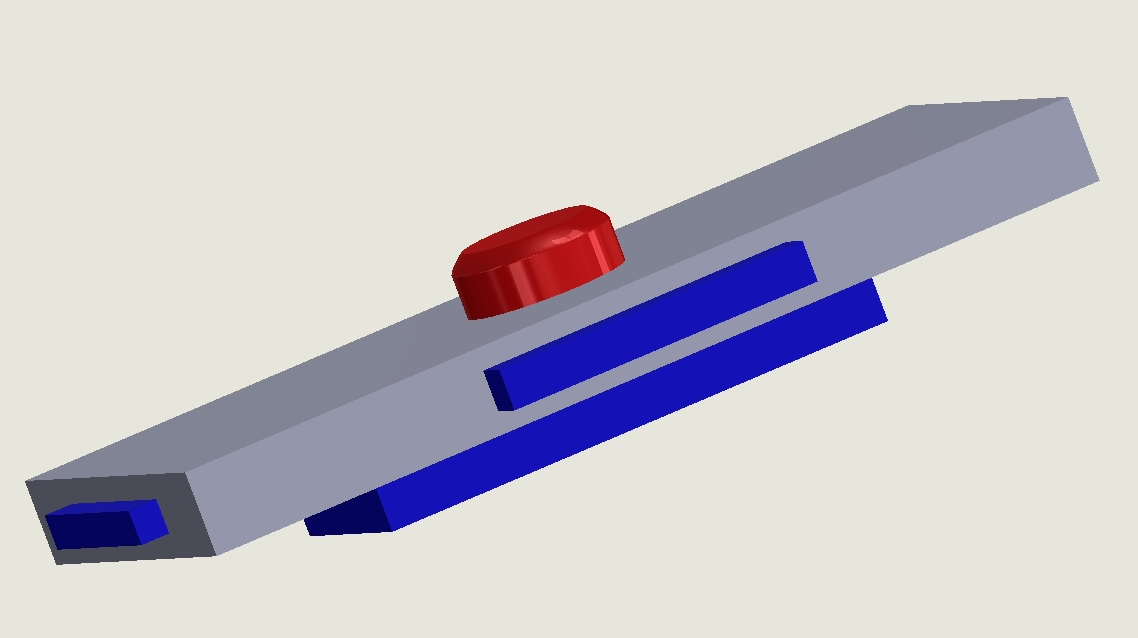
\includegraphics[width=0.8\textwidth]{Figures/Final.png}
  \caption{System Architecture}
  \label{fig:system_architecture}
\end{figure}

Where the microcontroller will be stored inside the box of the system and linked to the bluetooth module and the ultrasound sensors, which appear as blue boxes in Figure \ref{fig:system_architecture}, with the Gyroscope appearing with a Red Color.\\
The mounting of the circuit will be done as follows:
\begin{figure}[H]
  \centering

\tikzstyle{icdev}=[draw, text width=6em, minimum height=8em]

\begin{tikzpicture}[every node/.style = {font = \footnotesize},european]

    \node (digichip) [icdev,xshift=3cm,yshift=2cm] {};
    \draw (3.25,3.5) node(a1)[left]{$V_{cc}$};

    \draw (3.25,0.5) node(a2)[left]{GND};
    \draw (2.5,1.25) node(a3)[left]{A4};
    \draw (2.5,1.75) node(a4)[left]{A3};
    \draw (2.5,2.25) node(a5)[left]{A2};
    \draw (2.5,2.75) node(a6)[left]{A1};
    \draw (3.2,1.75) node(a7)[right]{D8};
    \draw (6.5,1.75) node(a8)[rectangle]{HM-10};
    \draw (0.5,2.75) node(a9)[left]{VL53L1X};
    \draw (0.5,2.25) node(a10)[left]{VL53L1X};
    \draw (0.5,1.75) node(a11)[left]{VL53L1X};
    \draw (0.5,1.25) node(a12)[left]{MPU650};
    \draw (2.75,-0.5) node(a13)[ground]{};
    \draw (3,4.5) node(a14)[left]{};
    \draw (a13) -- (a2);
    \draw (a14) -- (a1);
    \draw (a3) -- (a12);
    \draw (a4) -- (a11);
    \draw (a5) -- (a10);
    \draw (a6) -- (a9);
    \draw (a7) -- (a8);

\end{tikzpicture}

  \caption{Microcontroller Circuit}
  \label{fig:system_architecture}
\end{figure}
Only the pins that are used in the circuit have been shown in the Figure.
Unfortunately, it is not possible to simulate the circuit using popular circuit simulation software such as Proteus or Multisim, as either the MPU6050 or the Ultrasound sensors are not supported with the available libraries.
\tikzstyle{startstop} = [rectangle, rounded corners, 
minimum width=3cm, 
minimum height=1cm,
text centered, 
draw=black]
\tikzstyle{io} = [trapezium, 
trapezium stretches=true, % A later addition
trapezium left angle=70, 
trapezium right angle=110, 
minimum width=3cm, 
minimum height=1cm, text centered, 
draw=black]

\tikzstyle{process} = [rectangle, 
minimum width=4cm, 
minimum height=1cm, 
text centered, 
text width=3cm, 
draw=black]

\tikzstyle{decision} = [diamond, 
minimum width=2cm, 
minimum height=0.5mm,
text width= 8em, 
text centered, 
draw=black]
\tikzstyle{arrow} = [thick,->,>=stealth]
\subsection{Flowchart}
\begin{figure}[H]
\scalebox{0.8}[0.8]{
  \begin{tikzpicture}
    
    
      
    \node (start) [startstop] {Start};
  
    \node (p1) [process, below of=start, yshift=-1cm] {Input of the desired ranges of parameters of interest};
    \node (p2) [process, below of=p1, yshift= -1.5cm]{Signals are sent in predefined intervals};
    \node (p3) [process, below of=p2, yshift= -6.5cm]{The signals are then processed};
    \node (p4) [decision, below of=p3, yshift=-3.5cm]{Is W=0};
    \node (p5) [decision, below of=p4, xshift=-3cm, yshift=-2.5cm]{Is $S_{p} \notin R_{u} $};
    \node (p6) [process, below of=p5, yshift=-3cm]{W=1};
    \node (p7) [process, left of=p5, xshift=-4.5cm]{Do nothing};
    \node (p8) [startstop, left of=start, xshift=-2.5cm]{User end};
    \node (p9) [decision, below of=p4,xshift=3.5cm, yshift=-2.5cm]{Is $S_{p} \in R_{u} $};
    \node (p10) [process, below of=p9, yshift=-3cm]{W=0};
    \node (p11) [process, left of= p9,xshift=6cm]{Do nothing};
    \node (p12) [right of=p3, xshift=3cm]{};
    \node (p13) [right of= p2, xshift=3cm]{};
    \node (p14) [decision, below of=p2, yshift=-2.5cm]{Did the user input stop?};
    \node (p15) [process, left of =p3, xshift= -3.5cm]{Send parameters to the interface };
    \node (p16) [process, left of =p15, xshift= -3.5cm]{Display parameters on the interface};
    \draw [arrow] (start) -- (p1);
    \draw [arrow] (p1) -- (p2);
    \draw [arrow] (p2) -- (p14);
    \draw [arrow] (p3) -- (p4);
    \draw [arrow] (p4) -- node[anchor=east] {yes} (p5);
    \draw [arrow] (p5) -- node[anchor=east] {yes} (p6);
    \draw [arrow] (p5) -- node[anchor=north] {no} (p7);
    \draw [arrow] (p4) -- node[anchor=west] {no} (p9);
    \draw [arrow] (p9) -- node[anchor=east] {yes} (p10);
    \draw [arrow] (p9) -- node[anchor=north] {no} (p11);
    \draw [arrow] (p10) -| (p4);
    \draw [arrow] (p6) -|(p4);
    \draw (p3) -- (p12);
    \draw (p12) -- (p13);
    \draw [arrow] (p13) -- (p2);
    \draw [arrow] (p14) -| node[anchor=north] {yes} (p8);
    \draw [arrow] (p13) -- (p2);
    \draw [arrow] (p14) --node[anchor=west] {no} (p3);
    \draw [arrow] (p3) -- (p15);
    \draw [arrow] (p15) -- (p16);


  \end{tikzpicture}

}

  \caption{Algorithm of the system}
\end{figure}





\section{Calculations and Measurements}
The microcontroller will be responsible for taking the measurements from the sensors and performing the necessary calculations and sending the results to the user interface. The microcontroller will be responsible for the following:

\begin{itemize}
  \item \textbf{Distance Measurement:} The distance measurement will be straightforward, the microcontroller will be automatically given the distance between the sensor and the object in front of it with the time of flight of the ultrasound signal.
  \item \textbf{Velocity Measurement:} The velocity measurement will be done point by point to be able to draw a graph of the velocity across each axis. The velocity will be calculated straightforwadly by the taking the distance $\Delta d$ at a time $t_i$ between points $i-1$ and $i$ and dividing it by the time interval between two sent iterations.
    \begin{equation}
      v_i = \frac{\Delta d}{\Delta t}
    \end{equation}  
  \item \textbf{Acceleration Measurement:} The acceleration measurement will be done point by point to be able to draw a graph of the acceleration across each axis. The acceleration will be calculated straightforwadly by the taking the velocity $\Delta v$ at a time $t_i$between points $i-1$ and $i$ and dividing it by the time interval between two sent iterations.
    \begin{equation}
      a_i = \frac{\Delta v}{\Delta t}
    \end{equation}
  \item \textbf{Orientation Measurement:} The measurement of the orientation is a bit more complex, but by using a Gyroscope, we could be comparing the inclination of the quadcopter with a base value then calculate the error and send it to the user interface.
\end{itemize}

To ensure the maximization of the accuracy of the results, we will be computing the Position, Velocity, and Acceleration of the quadcopter in another way using the Accelerometer, using the following equations:
\begin{equation}
  \begin{aligned}
    \Delta x &= \frac{1}{2}a_x\Delta t^2 + v_x\Delta t \\
    \Delta v &= a_x\Delta t
  \end{aligned}
\end{equation}
These will be the combined with the results of the Ultrasonic Sensor to get the most accurate results.

\newpage
\section{Graphical User Interface}
The graphical user interface will be responsible for displaying the graphs of the parameters of the quadcopter, the user interface is separated into two windows:
\begin{itemize}
  \item \textbf{Main Plot Window:} The main plot window will be responsible for displaying the graphs of the parameters of the quadcopter.
    \begin{figure}[H]
    \centering
    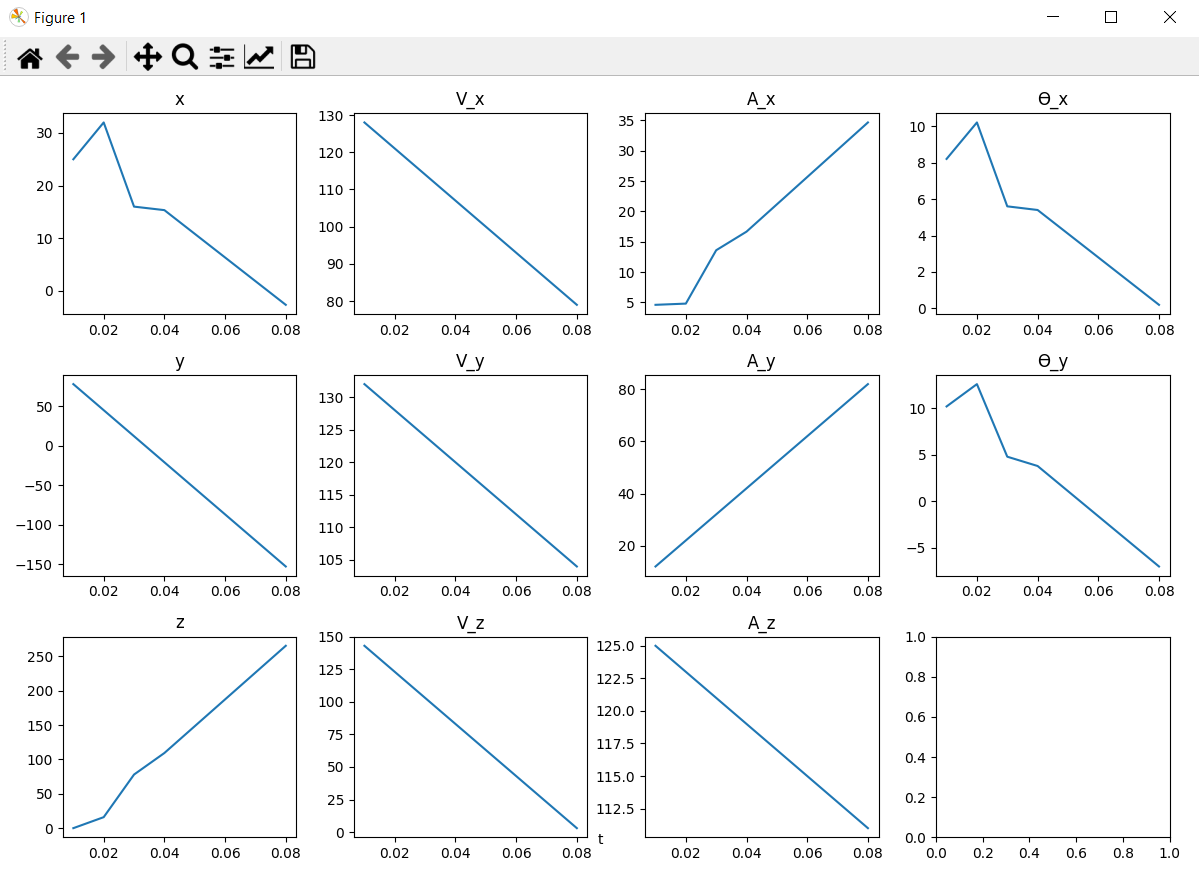
\includegraphics[width=0.8\textwidth]{Figures/PlotWindow.png}
    \caption{Main Plot Window}
  \end{figure}
  These graphs are updated in real time as the quadcopter travels.
  \item \textbf{Parameter Specification Window:} This window will be where the user inputs the minimum and maximum values of the parameters (ranges) for which they think the Quadcopter will be working, to be then alerted using LEDs and buzzers about the performance of the quadcopter not being within the specified ranges. Clicking on each parameter prompts a new window for which the user will be able to input their desired ranges.
    \begin{figure}[H]
    \centering
    \begin{subfigure}{0.45\textwidth}
      \centering
      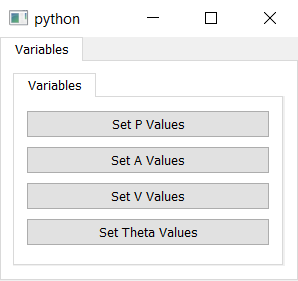
\includegraphics[width=\textwidth]{Figures/AllParam.png}
    \end{subfigure}
    \begin{subfigure}{0.45\textwidth}
      \centering
      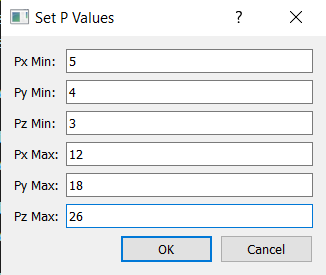
\includegraphics[width=\textwidth]{Figures/OneParam.png}
    \end{subfigure}
    \caption{Parameter Specification Window}
  \end{figure}
P refers to position, A to acceleration, and V to velocity, Theta is the angle of rotation (Pitch and Roll).\\
  The inputed ranges are stored in the local memory and communicated to the microcontroller using the serial port. The microcontroller will then be responsible for comparing the values of the parameters with the ranges and alerting the user using LEDs and buzzers.
  \begin{figure}[H]
    \centering
    
\includegraphics[width=0.8\textwidth]{Figures/ParamResult.png}
    \caption{Terminal Output Results after the input}
  \end{figure}
\end{itemize}
Note: All the used values are Dummy Data as we cannot synchronize the data without the hardware.

\newpage

\section{Sensor Fusion using Kalman Filters}
Since accelerometer and gyroscope sensors are both used together to determine the parameters (attitude) of the aircraft, we want to ensure that both of these sensors can have acceptable accuracy since the information required by the tester must be very precise. Combining both of them leads to deviation and the noise in the environment perturbates the sensing.
To overcome this problem, we will be using a Kalman Filter to fuse the data from both sensors to ensure that the data is as accurate as possible.\\
The Kalman Filter is a recursive algorithm that uses the previous state of the system to predict the next state of the system. It uses the measurements of the system to correct the prediction and ensure that the prediction is as accurate as possible.\\
We will be using a Kalman Filter library given by \cite{KalmanFilter} to implement the Kalman Filter in our system.\\
The Libraries have been modified accordingly and are integrated into the system as can be found in the GitHub repository linked in the Preface.\\






\section{Conclusion and Future Work}
    The graphical user interface, which makes up more than a quarter of the project implementation is already completed, and communication with the Microcontroller is already configured. In addition, the theoretical study of Kalman Filter which is the principal concept that is behind this project is also completed, with a good start in implementation in the code for the STM32 Microcontroller which will hopefully be completed once the parts are received. 
    The progress is definitely not as successful as we had hoped, but a lot of work was done from our part these last 2 weeks, which will hopefully smoothen the final part of the implementation to deliver an impeccable build.


   \newpage
    \appendix

    \section{Shipment Delay proofs}
    \begin{figure}[H]
      \centering
      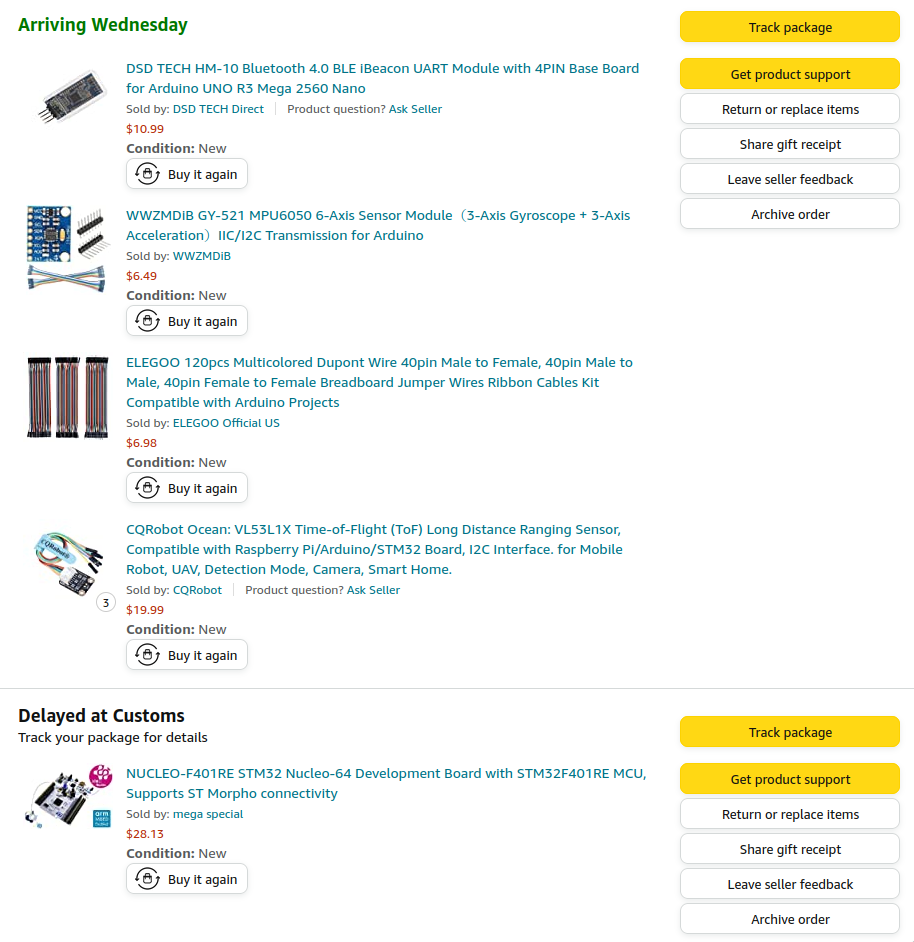
\includegraphics[width=0.5\textwidth]{Figures/Amazon.png}
    \end{figure}
    The Wednesday presented in the picture was supposed to be the 8th of March.
    \begin{figure}[H]
      \centering
      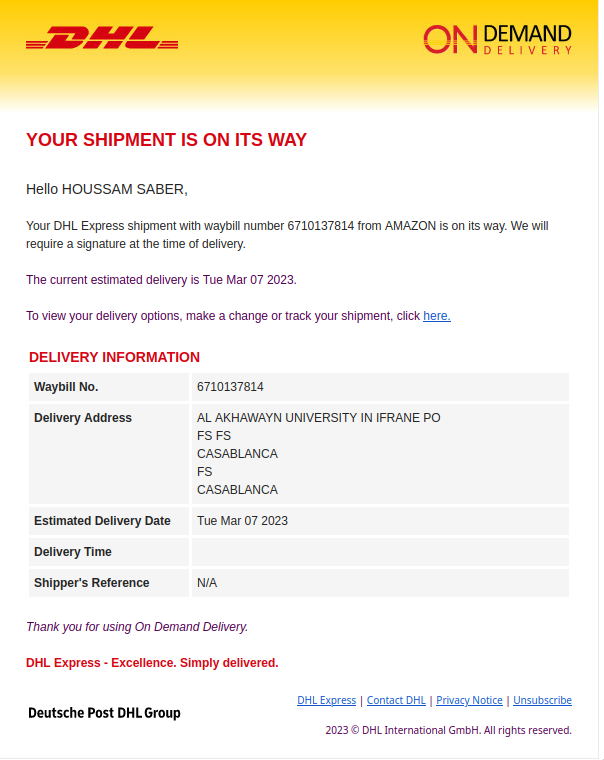
\includegraphics[width=0.5\textwidth]{Figures/DHL.png}
    \end{figure}





  \pagebreak
\bibliography{bibfile.bib}
\addcontentsline{toc}{section}{References}
\bibliographystyle{plain}
\nocite{*}





\end{document}
